\chapter{Resultados}\label{cap:Resultados}
A partir dos algoritmos implementados na biblioteca \textit{Komm}, foram realizados testes de compressão e descompressão com diferentes conjuntos de dados. Este capítulo apresenta os resultados obtidos, incluindo análises de desempenho e comparações com outras bibliotecas populares encontradas no github.

Para esta secção, foram utilizados 2 tipos de arquivos: arquivos de texto e arquivos de imagem. Os arquivos de texto foram escolhidos por serem comuns em aplicações de compressão, enquanto os arquivos de imagem foram selecionados para avaliar o desempenho.
Os arquivos utilizados foram:
\begin{itemize}
    \item \textbf{Arquivos de Texto:} Alice’s Adventures in Wonderland
    \item \textbf{Arquivos de Imagem:} Imagens no formato bitmap (BMP)
\end{itemize}
O arquivo de texto utilizado foi o livro "Alice’s Adventures in Wonderland", disponível no projeto Gutenberg\footnote{https://www.gutenberg.org/ebooks/11}. Este arquivo é representativo de textos literários e possui uma variedade de caracteres e padrões que são úteis para testar algoritmos de compressão.
As imagens no formatos .bmp podem ser vizuliadas na Figura \ref{fig:smiley} e \ref{fig:snail}.

\begin{figure}[h]
	\centering
	\caption{Imagem no formato bitmap (BMP) de um smiley}
	\label{fig:smiley}
	
\includegraphics[width=5cm]{figuras/smiley-large.png}
    \fonte{https://cse1.net/recaps/graphics}
\end{figure}

\begin{figure}[h]
	\centering
	\caption{Imagem no formato bitmap (BMP) de um caracol}
	\label{fig:snail}
	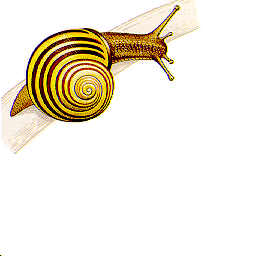
\includegraphics[width=5cm]{figuras/snail.png}
    \fonte{https://people.math.sc.edu/Burkardt/data/bmp/bmp.html}
\end{figure}

\pagebreak
\section{Métricas de Avaliação}
Para avaliar o desempenho dos algoritmos de compressão implementados na biblioteca \textit{Komm}, foram utilizadas as seguintes métricas:
\begin{itemize}
    \item \textbf{Taxa de Compressão:} A taxa de compressão é definida como a razão entre o tamanho do arquivo original e o tamanho do arquivo comprimido. Uma taxa de compressão maior indica uma melhor eficiência do algoritmo.
    \item \textbf{Tempo de Compressão e Descompressão:} O tempo gasto para comprimir e descomprimir os arquivos também foi medido. Tempos menores indicam um desempenho melhor do algoritmo.
    \item \textbf{Utilização de Memória:} A quantidade de memória utilizada durante o processo de compressão e descompressão foi monitorada para avaliar a eficiência do algoritmo em termos de recursos computacionais.
    \item \textbf{Integridade dos arquivos: } Após a descompressão, os arquivos foram comparados com os arquivos originais para garantir que não houve perda de dados durante o processo de compressão e descompressão.
\end{itemize}

\section{Resultados Obtidos}
